\subsection{Maurer's universal statistical test}
Maurer's universal test is one of the tests included in NIST SP 800-22 \cite{rukhin2001statistical,bassham2010sp}.
Maurer's universal statistical test aims at detecting non-randomness based on the test statistic value which is relating to the source's entropy, and the non-randomness is evaluated whether the computed entropy attains the maximum or not. 
%
Unlike other types of statistical tests which is designed to detect specific defects, Maurer's universal test is able to detect a wide range of statistical defects.
%
\par
Let us consider an information source $S$ which generates a sequence $U_1,U_2,\dots$. For each $i$, we regard $U_i$ as a sample from a random variable.
A source $S$ is called a finite memory source if there exists a positive integer $M$ such that the conditional probability of $U_n$, given $U_1,\dots,U_{n-1}$, depends only on the most previous $M$ bits, i.e.,
\begin{align}\label{eq:memory}
	P_{U_n\mid U_{n-1}\dots U_{1}}(u_n \mid u_{n-1}\dots u_{1}) = P_{U_n\mid U_{n-1}\dots U_{n-M}}(u_n \mid u_{n-1}\dots u_{n-M}),
\end{align}
for $n>M$ and for every binary sequence $u_1,\dots,u_n\in\{0,1\}^n$. The smallest $M$ satisfying Eq. (\ref{eq:memory}) is called the memory of the source. The probability distribution of $U_n$ is thus determined by the source's state $\Lambda_n = U_{n-M},\dots,U_{n-1}$ at time $n$. Let $\Lambda_1 = U_0 \dots U_{-M+1}$ be the initial state where $U_{-M+1}\dots U_0$ are dummy random variables. Then, the source is called \textit{stationary}, if the information source $S$ satisfies the following relation in addition to Eq. (\ref{eq:memory}),
\begin{align}
	P_{U_n\mid\Lambda_n}(u\mid \lambda) = P_{U_1\mid\Lambda_1}(u\mid \lambda),
\end{align}
for all $n>M$, $u\in\{0,1\}$ and $\lambda \in \{0,1\}^M$. 
%
Therefore, it depends only on the most previous $M$-bit sequence when a sequence is generated by a stationary source.
%
On the other hand, each bit is independent of the previous sequence, and the probability of taking ``$1$'' or ``$0$'' is exactly the same as $\frac{1}{2}$ if we say a sequence is truly random in intuitive sense.
%
\par
%
The formulation of Maurer's universal test is motivated by the universal source coding algorithms that has been proposed in \cite{elias1987interval,willems1989universal} and the procedure is described as follows. In the following, let $B$ be the set $\{0,1\}$, and $x^n = x_1,x_2,\dots,x_n \in B^n$ be a binary sequence of length $n$, where $x_i\in B$. The test takes as input three positive integers $L,\,Q$ and $K$, and a binary sequence $s^n \in B^n$ generated by a tested source. The sequence is divided into adjacent non-overlapping blocks of length $L$. Then, the first $Q$ blocks ($L\times Q$-bits) are used for initialization, and the remaining $K$ blocks ($L\times K$-bits) are used for the test. Without loss of generality, we can assume that $n=L\times(Q+K)$ holds\footnote{%
If the relation $n=L\times(Q+K)$ does not hold, then let $K$ be $\left\lfloor \frac{n}{L} \right\rfloor - Q$.
}. 
%
Let $b_k(x^n)$ be the $k$-th block of $x^n$, i.e., $b_k(x^n) = x_{L(k-1)+1}, x_{L(k-1)+2}, \dots, x_{Lk}$. Considering the situation that the $(n-m)$-th block takes the same value with the $n$-th block and the blocks from $(n-m+1)$-th to $(n-1)$-th blocks do not take the value, we define an integer-valued variable $A_n(x^n)$ as $m$. 
Figure \ref{fig:A_n_example} illustrates an example for $L=3$. The test function $f_M$, which maps a binary sequence to a real number, is defined by 
\begin{align}\label{eq:fM}
	f_M(x^n) = \frac{1}{K} \sum_{n=Q+1}^{Q+K} \log_2 A_n(x^n),
\end{align}
where $A_n(x^n)$ is defined by
\begin{align}\label{eq:An}
	A_{n}(x^n) = \left\{ \begin{array}{ll}
	n, \quad \text{if} \:\: b_{n-m}(x^n) \neq b_n(x^n) \:\: \text{for} \:\: 1 \leq m \leq n-1, \\
	\min \{ m\in\mathbb{N} \mid m \geq 1,\, b_{n-m}(x^n) = b_n(x^n) \}, \quad \text{otherwise},
	\end{array} \right.
\end{align}
for $n=Q+1,Q+2,\dots,Q+K$.
%-------------------------------------------------------------------
\begin{figure}
\centering
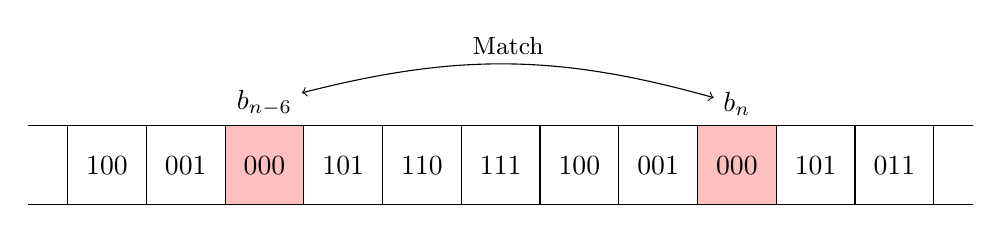
\begin{tikzpicture}
\draw (-1.5,0)--(-1.0,0);
\draw (-1.5,1)--(-1.0,1);
\draw (-1.0,0) rectangle (0,1) node at (-0.5, 0.25) [above] {$100$};
\draw (0,0) rectangle (1,1) node at (0.5, 0.25) [above] {$001$};
\filldraw [draw=black, fill=pink] (1,0) rectangle (2,1) node at (1.5, 0.25) [above] {$000$} node (A) at (1.5, 1.0) [above] {$b_{n-6}$};
\filldraw [draw=black, fill=white] (2,0) rectangle (3,1) node at (2.5, 0.25) [above] {$101$} ;
\filldraw [draw=black, fill=white] (3,0) rectangle (4,1) node at (3.5, 0.25) [above] {$110$};
\filldraw [draw=black, fill=white] (4,0) rectangle (5,1) node at (4.5, 0.25) [above] {$111$};
\filldraw [draw=black, fill=white] (5,0) rectangle (6,1) node at (5.5, 0.25) [above] {$100$};
\filldraw [draw=black, fill=white] (6,0) rectangle (7,1) node at (6.5, 0.25) [above] {$001$};
\filldraw [draw=black, fill=pink] (7,0) rectangle (8,1) node at (7.5, 0.25) [above] {$000$} node (AA) at (7.5, 1.0) [above] {$b_n$};
\draw (8,0) rectangle (9,1) node at (8.5, 0.25) [above] {$101$};
\draw (9,0) rectangle (10,1) node at (9.5, 0.25) [above] {$011$};
\draw (10,0)--(10.5,0);
\draw (10,1)--(10.5,1);
%
\draw[<->] (A) to[bend left=15] node [above] {\small Match} (AA);
\end{tikzpicture}
\caption{An example of the situation of $A_n=6$ for $L=3$.}
\label{fig:A_n_example}
\end{figure}
%-------------------------------------------------------------------
%
\par
%
In order to evaluate the non-randomness of a given binary sequence, it is necessary to derive the expected value and the variance of the reference distribution for a truly random sequence. Note that a truly random sequence is a binary sequence generated by a uniform distribution on $\{0,1\}^n$. 
Under the assumption $Q\to\infty$, the expectation and the variance are given by
\begin{align}
	\mathbb{E}[f_M(R^n)]  &= 2^{-L}\sum_{i=1}^{\infty}(1-2^{-L})^{i-1} \log_2 i \label{eq:mean_maurer},\\
	\sigma_M^2 &= c_M(L,K)^2 \times \frac{\mathrm{Var}[\log_2 A_n(R^n)]}{K} \label{eq:sigma_maurer},
\end{align}
%
where $R^n$ denotes a truly random sequence of length $n$. 
%
In \cite{maurer1992universal}, the following approximation is empirically proposed:
\begin{align}\label{eq:cM_maurer}
	c_M(L,K) \simeq 0.7 - \frac{0.8}{L} + \left( 1.6 + \frac{12.8}{L} \right) K^{-4/L}.
\end{align}
The approximation above has been obtained by numerical simulations. 
%
In \cite{coron1998accurate}, the accurate expression of $c_M(L,K)$ has been obtained theoretically. 
However, it requires much cost to compute the $c_M(L,K)$ for given $L$ and $K$, and hence an approximation of the theoretical form is given as follows:
\begin{align}\label{eq:cM_coron}
	c_M(L,K)^2 \simeq d_M(L) + \frac{e_M(L)\times2^L}{K}, 
\end{align} 
where $d_M(L)$ and $e_M(L)$ are listed in \cite{coron1998accurate} for $L=3,4,\dots,16$. 
The approximation in Eq. (\ref{eq:cM_coron}) is accurate for $K\geq 33\times 2^L$ in practice.
%
Note that $\mathrm{Var}[\log_2 A_n]$ in Eq. (\ref{eq:sigma_maurer}) can be computed by the definition of variance by
\begin{align}
 	\mathrm{Var}[\log_2 A_n(R^n)] = 2^{-L}\sum_{i=1}^{\infty}(1-2^{-L})^{i-1} (\log_2 i)^2 - (\mathbb{E}[f_M(R^n)])^2.
\end{align}
%
\par
%
To implement the test, it is necessary to set the parameters. In \cite{maurer1992universal}, the study recommends to set parameters $L\,Q$ and $K$ as $6\leq L,\, \leq 16$, $Q \geq 10 \times 2^L$ and $K \geq 1000\times 2^L$, respectively. 
%
The study also insists that rejection rate $\rho$ should be chosen as $\rho \in [0.001, 0.01]$. 
%
Then, it is concluded that the null hypothesis of Maurer's test\footnote{A null hypothesis of Maurer's test is that a binary sequence of length $n$ follows a uniform distribution on $\{0,1\}^n$} 
is rejected if either $f_M(x^n)<t_1$ or $f_M(x^n)>t_2$ holds, where the thresholds $t_1$ and $t_2$ are written as
\begin{align}\label{eq:ysigma}
\begin{split}
	t_1 &= \mathbb{E}[f_M(R^n)] - y\sigma_M, \\
	t_2 &= \mathbb{E}[f_M(R^n)] + y\sigma_M.
\end{split}
\end{align}
Using the complementary error function $\mathrm{erfc}$ defined by
\begin{align}
   \text{erfc}(z) = \frac{2}{\sqrt{\pi}} \int_{z}^{\infty} \mathrm{e}^{-u^2} \, \mathrm{d}u,
\end{align}
the value $y$ in Eq. (\ref{eq:ysigma}) is given as $\mathrm{erfc}(y)=\frac{\rho}{2}$. 
Notice that it is implicitly assumed that $f_M(R^n)$ follows a normal distribution.
%
\par
In NIST SP 800-22, the non-randomness is evaluated by the p-value shown as
\begin{align}
	p\mathchar`- \mathrm{value}_M 
	% p_M
	= \mathrm{erfc} \left( \left| \frac{f_M(x^n) - \mathbb{E}[f_M(R^n)]}{\sqrt{2} \sigma_M} \right| \right),
\end{align}
where $\mathrm{erfc}$ is the complementary error function defined by
Then, the null hypothesis of Maurer's test is rejected if $p\mathchar`- \mathrm{value}_M < \alpha$, where $\alpha$ is a significance level.
%-------------------------------------------------------------------
\par
There is much concern in the asymptotic relation between the Maurer's test statistic and the source's per-bit entropy. In \cite{maurer1992universal}, the expected value of the test statistic for a truly random sequence $\mathbb{E}[f_M(R^n)]$ is closely related to the entropy of blocks. It has been shown that the following relation holds:
\begin{align}\label{eq:maurer_asymptotic_R}
	\lim_{L\to\infty} \left[ \mathbb{E}[f_M(R^n)] -L \right] = C,
\end{align}
where $C$ is a constant whose value is equal to $-\frac{\ln 2}{\gamma} \simeq -0.8327$ and $\gamma$ is Euler's constant \cite{hardy1979introduction}. We provide the proof of $C=-\frac{\ln 2}{\gamma}$ is given in Appendix \ref{appendix:A}. 
%
Let us consider a binary sequence $U_{\mathrm{BMS}_p}^n$ generated by a binary memoryless source $\mathrm{BMS}_p$. Note that a sequence $U_{\mathrm{BMS}_p}^n$ follows a distribution on $\{0,1\}^n$ taking each bit to be ``$1$'' with probability $p\in (0,1)$ independently. 
%
For a binary sequence $U_{\mathrm{BMS}_p}^n \in B^n$, the following relation
\begin{align}
	\lim_{L\to\infty} \left[ \mathbb{E}[f_M(U_{\mathrm{BMS}_p}^n)] -L\times H(p) \right] = C
\end{align}
holds for any $p \in (0,1)$, where $H$ is the binary entropy function corresponding to $\mathrm{Pr}[X=1]=p$. Here, $X$ is a random variable. 
%
In \cite{maurer1992universal}, a similar result has been studied to show for a binary sequence $U_s^n$ generated by every ergodic stationary source $S$. The study in \cite{coron1998accurate} develops the idea and proves that the following relation holds:
\begin{align}
	\lim_{L\to\infty} \left[ \mathbb{E}[f_M(U_s^n)] - K_L \right] = C,
\end{align}
where $K_L$ is equivalent to the entropy of $L$ bit blocks defined by
\begin{align}\label{eq:K_L}
	K_L = -\sum_{b \in B^n} \mathrm{Pr}[b] \log_2 \mathrm{Pr}[b].
\end{align}
Other asymptotic relations between Maurer's test statistic and a source's entropy can be found in \cite{wegenkittl2001entropy,choe2000average,abadi2004version,kim2014estimation,kim2018low}.
%-------------------------------------------------------------------%
%-------------------------------------------------------------------%
%-------------------------------------------------------------------%
%-------------------------------------------------------------------%
%-------------------------------------------------------------------%
%-------------------------------------------------------------------%
%-------------------------------------------------------------------%
%-------------------------------------------------------------------%
%-------------------------------------------------------------------%
%-------------------------------------------------------------------%
%-------------------------------------------------------------------%
%-------------------------------------------------------------------%
%-------------------------------------------------------------------%
\subsection{Coron's universal statistical test}
As seen in the previous subsection, Maurer's universal test can detect a wide range of statistic defects modeled by an ergodic statistic source with finite memory, however, the test only provides an asymptotic measure of the source's entropy. 
%
To address the problem, a modified version of Maurer's universal test called ``Coron's universal test'' has been proposed in \cite{coron1999security}. In this test, the expectation of test statistic value is exactly equal to the source's entropy. The main procedure is the same as Maurer's test except for the test statistic. The test function $f_C$, which maps a binary sequence to a real number, is defined by 
\begin{align}\label{eq:fC}
	f_C(x^n) = \frac{1}{K} \sum_{n=Q+1}^{Q+K} g(A_n(x^n)),
\end{align}
where $A_n(x^n)$ is defined by Eq. (\ref{eq:An}) and $g:\mathbb{N}\to\mathbb{R}$ is given by
\begin{align}\label{eq:function_g}
	g(m) = (\log_2 \mathrm{e}) \sum_{k=1}^{m-1}\frac{1}{k},
\end{align}
for $m\geq 2$. Note that we set $g(1)=0$.
%
For a binary sequence $U_s^n$ generated by an ergodic stationary source $S$, the expected value is exactly equal to the entropy of $L$ blocks of $S$, i.e.,
\begin{align}\label{eq:coron_expected_value_for_U}
	\mathbb{E}[f_C(U_s^n)] = K_L,
\end{align}
where $K_L$ corresponds to the entropy of blocks given by Eq. (\ref{eq:K_L}).
%
\par
It is necessary to derive the expected value and the variance of the reference distribution just like Maurer's test. From Eq. (\ref{eq:coron_expected_value_for_U}), the expected value for $R^n$ is obtained by
\begin{align}
\label{eq:coron_expected_value_truly_random}
	\mathbb{E}[f_C(R^n)] &= L, 
\end{align}
since $K_L=L$ when the source is the binary symmetric source. 
The variance is also obtained as
\begin{align}
	\sigma_C^2 &= c_C(L,K)^2 \times	\frac{\mathrm{Var}[g(A_n)]}{K}.
\end{align}
In \cite{coron1999security}, the following approximation is empirically proposed as
\begin{align}
	c_C(L,K) \simeq d_C(L) + \frac{e_C(L)\times 2^L}{K},
\end{align}
where $d_C(L)$ and $e_C(L)$ are listed in \cite{coron1999security} for $L=3,4,\dots,16$.
Note that $\mathrm{Var}[g(A_n)]$ can be calculated by the definition of variance as
\begin{align}
\begin{split}
	\mathrm{Var}[g(A_n)] 
	&= \mathbb{E}[\{g(A_n)\}^2] - \left( \mathbb{E}[g(A_n)] \right)^2 \\
	&=2^{-L} \sum_{i=2}^{\infty} (1-2^{-L})^{i-1} \left( \sum_{k=1}^{i-1} \frac{\log_2 \mathrm{e}}{k} \right)^2 -L^2.
\end{split}
\end{align}
To obtain the second equality in the above equations, we use the relation $\mathbb{E}[g(A_n)]=\mathbb{E}[f(x^n)]=L$.
%
When we consider a binary sequence $U_{\mathrm{BMS}_p}^n$ generated by a binary memoryless source $\mathrm{BMS}_p$, we exactly have
\begin{align}\label{eq:E_BMS}
	\mathbb{E}[f_C(U_{\mathrm{BMS}_p}^n)] = L\times H(p).
\end{align}
%
%-------------------------------------------------------------------%
%-------------------------------------------------------------------%
%-------------------------------------------------------------------%
%-------------------------------------------------------------------%
%-------------------------------------------------------------------%
%-------------------------------------------------------------------%
%-------------------------------------------------------------------%
%-------------------------------------------------------------------%
%-------------------------------------------------------------------%
%-------------------------------------------------------------------%
%-------------------------------------------------------------------%
\subsection{Highly sensitive universal statistical test}
In the previous subsections, we have seen that Maurer's and Coron's universal statistical test can detect the non-randomness of a binary sequence.
Both tests evaluate the non-randomness of a binary sequence whether the relation (\ref{eq:maurer_asymptotic_R}) or (\ref{eq:coron_expected_value_truly_random}) holds for $p=0.5$, where $q=\mathrm{Pr}[x_i=1]$. It has been suggested in \cite{yamamoto2016highly} that the deviation from $p=0.5$ cannot be detected with high sensitivity since the derivative of the binary entropy function is equal to $0$ at $p=0.5$, i.e.,
\begin{align}
  \left.\frac{\mathrm{d}}{\mathrm{d}p}H(p) \right|_{p=0.5} = \left.\log_2\frac{1-p}{p}\right|_{p=0.5} = 0.
\end{align}
\par
In \cite{yamamoto2016highly}, the universal test called ``highly sensitive universal statistical test'' has been proposed. This test is constructed on the basis of Maurer's and Coron's universal statistical tests.
%
In the highly sensitive test, a given binary sequence $x_1,x_2,\dots$ with $q \simeq 0.5$ is converted into another binary sequence $\hat{x}_1,\hat{x}_2,\dots$ with $\hat{q} \neq 0.5$ by
%
\begin{align}\label{eq:convert}
\begin{split}
  \mathrm{Pr}[\hat{x}_i = 0 \mid x_i=0] &= 1, \\
  \mathrm{Pr}[\hat{x}_i = 1 \mid x_i=1] &= \beta,
\end{split}
\end{align}
%
where $\hat{q}=\mathrm{Pr}[\hat{x}_i=1]$ and $\beta \in (0,1)$. Note that ``$0$'' in a sequence is not converted, and ``$1$'' in a sequence is flipped into ``$0$'' in probability with $1-\beta$. By Eq. (\ref{eq:convert}), a given sequence is converted into another binary sequence with $\hat{q}=0.5\beta$. In \cite{yamamoto2016highly}, the non-randomness can be detected by applying Coron's universal test for a converted binary sequence.
Numerical experiments show the effectiveness of the highly sensitive test and $\beta=0.66$ maximizes the effectiveness.
%
\par
The null hypothesis under the highly sensitive test $\mathcal{H}_0$ is that a binary sequence of length $n$ being tested follows a uniform distribution on $\{0,1\}^n$. As an implicit assumption, an additional hypothesis $\widetilde{\mathcal{H}}_0$ that a random number used for flipping is ideal needs to be considered. Hence, the null hypothesis under the highly sensitive test $\overline{\mathcal{H}}_0:=\mathcal{H}_0 \land \widetilde{\mathcal{H}}_0$ is that a converted binary sequence is considered to be generated by a distribution on $\{0,1\}^n$ taking each bit to be ``$1$'' with probability $\hat{q}$ independently. If the null hypothesis $\overline{\mathcal{H}}_0$ is rejected, then the hypothesis $\mathcal{H}_0$ would be rejected. Otherwise, there is no evidence for rejecting the null hypothesis $\overline{\mathcal{H}}_0$. The algorithm of the highly sensitive test is described in Algorithm \ref{alg:highly}.
%
\begin{algorithm}[h]
\caption{The procedure of highly sensitive universal statistical test}
\label{alg:highly}
\begin{algorithmic}[1]
\State Set parameters $\alpha,\,L,\, Q,\,K$ and $\beta$.
\State Convert a given binary sequence $s^n$ into $\hat{s}^n$ by Eq. (\ref{eq:convert}).
\State Divide a converted binary sequence $\hat{s}^n$ into adjacent non-overlapping blocks of length $L$, and compute $A_n(\hat{s}^n)$ for $n=Q+1,Q+2,\dots,Q+K$ by Eq.(\ref{eq:An}). \label{state:divide}
\State Compute a test statistic value $f_C(\hat{s}^n)$ by Eq. (\ref{eq:fC}).
\State Compute a $p \, \mathchar`- \mathrm{value}$ by
\begin{align}
	 p\mathchar`- \mathrm{value} = \mathrm{erfc} \left( \left| \frac{f_C(\hat{s}^n) - L\times H(0.5\beta)}{\sqrt{2} \sigma_C(0.5\beta)} \right| \right).
\end{align}
\State Reject $\mathcal{H}_0$ if $p\mathchar`- \mathrm{value} < \alpha$; else accept $\overline{H}_0$.
\end{algorithmic}
\end{algorithm}
%
\par
%
To implement the highly sensitive test, it is necessary to derive the expected value and the variance of reference distribution of a binary sequence.
%
By Eq. (\ref{eq:E_BMS}), the expected value has been obtained, whereas the variance has not been analyzed theoretically. Then, a value obtained by simulation is used as the variance in \cite{yamamoto2016highly}. The accurate variance should be derived to improve the reliability of the highly sensitive test.
%-------------------------------------------------------------------%
%-------------------------------------------------------------------%
%-------------------------------------------------------------------%
%-------------------------------------------------------------------%
%-------------------------------------------------------------------%
%-------------------------------------------------------------------%
%-------------------------------------------------------------------%
%-------------------------------------------------------------------%
%-------------------------------------------------------------------%
%-------------------------------------------------------------------%
%-------------------------------------------------------------------%
%-------------------------------------------------------------------%
%-------------------------------------------------------------------%
%-------------------------------------------------------------------%
%-------------------------------------------------------------------%
%-------------------------------------------------------------------%
%-------------------------------------------------------------------%
%-------------------------------------------------------------------%
%-------------------------------------------------------------------%
%-------------------------------------------------------------------%
%-------------------------------------------------------------------%